\usetikzlibrary{arrows}
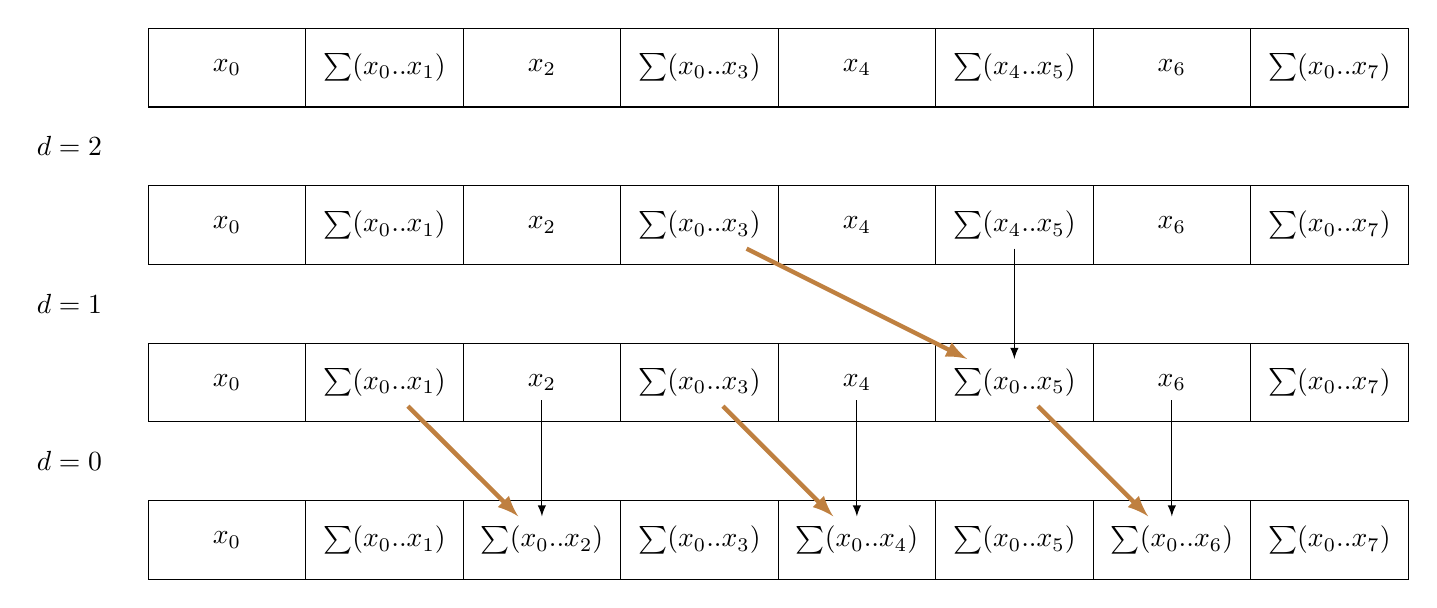
\begin{tikzpicture}

\draw (0,0) rectangle +(16,1);
\draw (0,2) rectangle +(16,1);
\draw (0,4) rectangle +(16,1);
\draw (0,6) rectangle +(16,1);

\foreach \y in {0,2,4,6}
\foreach \x in {2,4,...,15} {
	\draw (\x,\y) -- +(0,1);
}

% levels
\node at (-1,1.5) {$d=0$};
\node at (-1,3.5) {$d=1$};
\node at (-1,5.5) {$d=2$};

\node (v12) at (1,0.5) {$x_0$}; \node (v16) at (1,2.5) {$x_0$}; \node at (1,4.5) {$x_0$}; \node at (1,6.5) {$x_0$};
\node (v1) at (3,0.5) {$\sum(x_0..x_1)$}; \node (v2) at (3,2.5) {$\sum(x_0..x_1)$}; \node at (3,4.5) {$\sum(x_0..x_1)$}; \node at (3,6.5) {$\sum(x_0..x_1)$};
\node (v13) at (5,0.5) {$\sum(x_0..x_2)$}; \node (v21) at (5,2.5) {$x_2$}; \node at (5,4.5) {$x_2$}; \node at (5,6.5) {$x_2$}; 
\node (v3) at (7,0.5) {$\sum(x_0..x_3)$}; \node (v4) at (7,2.5) {$\sum(x_0..x_3)$}; \node (v11) at (7,4.5) {$\sum(x_0..x_3)$}; \node (v17) at (7,6.5) {$\sum(x_0..x_3)$};
\node (v14) at (9,0.5) {$\sum(x_0..x_4)$}; \node (v20) at (9,2.5) {$x_4$}; \node at (9,4.5) {$x_4$}; \node at (9,6.5) {$x_4$};
\node (v5) at (11,0.5) {$\sum(x_0..x_5)$}; \node (v6) at (11,2.5) {$\sum(x_0..x_5)$}; \node (v18) at (11,4.5) {$\sum(x_4..x_5)$}; \node at (11,6.5) {$\sum(x_4..x_5)$};
\node (v15) at (13,0.5) {$\sum(x_0..x_6)$}; \node (v19) at (13,2.5) {$x_6$}; \node at (13,4.5) {$x_6$}; \node at (13,6.5) {$x_6$};
\node (v7) at (15,0.5) {$\sum(x_0..x_7)$}; \node (v8) at (15,2.5) {$\sum(x_0..x_7)$}; \node (v9) at (15,4.5) {$\sum(x_0..x_7)$}; \node (v10) at (15,6.5) {$\sum(x_0..x_7)$};

%\draw [-latex] (v10) edge (v9);
\draw [-latex, ultra thick, brown] (v11) edge (v6);

\draw [-latex, ultra thick, brown] (v6) edge (v15);
\draw [-latex, ultra thick, brown] (v4) edge (v14);
%\draw [-latex] (v9) edge (v8);
%draw [-latex] (v8) edge (v7);
%\draw [-latex] (v6) edge (v5);
%\draw [-latex] (v11) edge (v4);
%\draw [-latex] (v4) edge (v3);
\draw [-latex, ultra thick, brown] (v2) edge (v13);
%\draw [-latex] (v2) edge (v1);

\draw [-latex] (v18) edge (v6);
\draw [-latex] (v19) edge (v15);
\draw [-latex] (v20) edge (v14);
\draw [-latex] (v21) edge (v13);
%\draw [-latex] (v16) edge (v12);
\end{tikzpicture}